\chapter{Information Extraction}

To calculate the similarity between a job and a resume, the JobFinder system needs structured digital models of each document. To get the structured data, some JRSs ask the job seekers input their profiles in forms field by field, and the recruiter input their job descriptions in the same way. However, as we discussed in Chapter 2, the users are reluctant to take the tedious process~\cite{singh2010prospect}. Job seekers prefer upload their resumes directly, and recruiters prefer to post the whole job descriptions to web sites.

In this chapter we will explain how the Information Extraction (IE) module of our system extracts information from these unstructured data source. An example of job description is shown in Table~\ref{tab:jd1}. The IE framework will be introduced by example of processing the job descriptions. The Finite-State Transducer(FST) library, which is used as pattern matching tools, will be introduced as well.

\begin{table}[!p]
 \small
\caption{Example of Job Description} % title of Table
\centering % used for centering table
\begin{tabular}{    |  p{15cm} |  }
\hline
\\
\large{\textbf {Senior/Principal Software Engineer}}\\
RichRelevance - San Francisco, CA \\
\\

RichRelevance powers personalized shopping experiences for the world��s largest and most innovative retail brands, including Target, Sears, Marks \& Spencer, John Lewis and others. Founded and led by the e-commerce expert who helped pioneer personalization at Amazon.com, RichRelevance helps retailers increase sales and customer engagement by recommending the most relevant content to consumers regardless of the channel they are shopping. RichRelevance has delivered more than \$5.5 billion in attributable sales for its retail clients to date, and is accelerating these results with the introduction of a new form of digital advertising called Shopping Media which allows manufacturers to engage shoppers where it matters most -- in the digital aisles on the largest retail sites in world. RichRelevance is headquartered in San Francisco, with offices in New York, Seattle, Boston, Reading and Malmho, and has been twice recognized as one of the ��Best Places to Work�� in the Bay Area.
\\
RichRelevance is looking for a Senior/Principal Software Engineer to join our growing team! \\

\textbf{Primary responsibilities:} \\
~~~~~~$\bullet$ Working with large scale distributed systems \\
~~~~~~$\bullet$ Work with Hadoop ecosystem (technologies like Hive, Impala, HBase) \\
~~~~~~$\bullet$ Algorithmic development with primary focus Machine Learning \\\
~~~~~~$\bullet$ Working with rapid and innovative development methodologies like: Kanban, Continuous Integration and Daily deployments \\
~~~~~~$\bullet$ Unit testing with JUnit, Performance testing and tuning\\
\\
\textbf{Minimum requirements:} \\

~~~~~~$\bullet$ BS/MS in CS, Electrical Engineering or foreign equivalent plus relevant software development experience \\
~~~~~~$\bullet$ At least 5+ years of software development experience \\
~~~~~~$\bullet$ Expert in Java, Scala or any other object oriented language \\
~~~~~~$\bullet$ Proficient in SQL concepts (HiveQL or Postgres a plus) \\
~~~~~~$\bullet$ Additional language skills for scripting and rapid application development\\
\\
\textbf{Desired skills and experience:}\\
~~~~~~$\bullet$ Working with large data sets in the PBs \\
~~~~~~$\bullet$ Familiarity with UNIX (systems skills a plus) \\
~~~~~~$\bullet$ Working in a distributed environment and has dealt with challenges around scaling and performance \\
~~~~~~$\bullet$ Mobile development for Android or iOS.\\
\\
RichRelevance is an Equal Opportunity Employer and does not discriminate against any applicant on the basis of race, color, religion, national origin, gender, marital status, age, disability, sexual orientation, military/veteran status, or any other status protected by Federal or State law or local ordinance.
\\
\hline

\end{tabular}
\label{tab:jd1} % is used to refer this table in the text
\end{table}


\section{Text Processing Stages}

Information Extraction is the task of automatically extracting structured information such as entities, relationships between entities, and attributes describing entities from unstructured sources~\cite{sarawagi2008information}. The IE framework in our system uses six stages in order to extract the information from job descriptions: HTML parsing, segmenting, preprocessing, tokenizing, labeling and pattern matching, which is show in Figure~\ref{fig:Pipeline}.

1) The \textbf{HTML Parsing} will parse the web pages that contain job descriptions, which are obtained from web crawler. The parser uses HTML tag template to extract attributes of the jobs, like job title, location, company name, content and so on. A job will be saved as a record with these attributes in the database. In the record, the content field contains the text part of the job description, which will be processed in later stages.

2) In the \textbf{segmenting stage}, the content field of the job description is be separated into paragraphs according HTML tags. Then paragraphs are separated into sentences by either HTML tags or punctuation, and after this step, all HTML tags will be removed.

3) Web pages of job description are created in different character sets, (e.g. UTF8 and ISO 8859-1), and almost always contain some unreadable characters. In the \textbf{prepossessing stage}, characters in the sentences are converted to ASCII characters, unreadable characters will be deleted, and some punctuation will be replaced by spaces (e.g. / and -).

4) In the \textbf{tokenizing stage}, the sentences will be tokenized into arrays of tokens by NLTK~\cite{bird2006nltk}.

5) In the \textbf{labeling stage}, the sentences will be given two layers of labels by a dictionary matching approach. The labels in the first layer are the semantic value of the text, and the labels in the second layer are the ontology hypernym of the labels in the first layers.

6) In the \textbf{pattern matching} stage, the FST library is used to matching the labels of the labeled sentences.  If a layered sentence match any pre-defined pattern, the information will be extracted and added to the job model. After every sentence of a job description has be processed, a job model will be created and saved in the database. More details about matching will follow in Section C.

\begin{figure}[htbp]
  \centering
  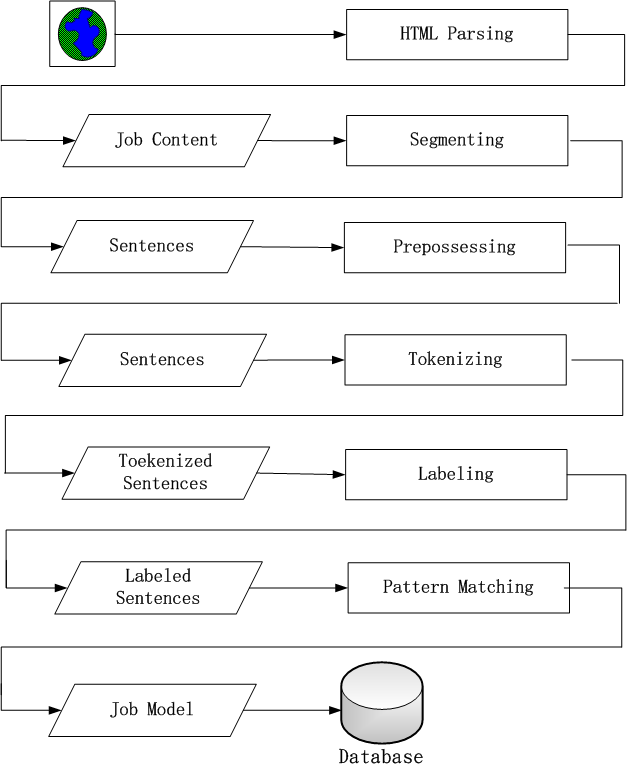
\includegraphics[scale=0.4]{images/pipeline2.png}
  \caption{Job Description Process Pipeline}
  \label{fig:Pipeline}
\end{figure}

\section{Semantic Labeling}

In this section, we will introduce why and how we add two layers of label to the tokenized sentences. In natural language, a single concept often has multiple expressions o represent it. For example, the simple concept bachelor's degree,  can be expressed in many ways in job descriptions, e.g. B.S., BA/BS, 4-years-degree, and so on. Table \ref{tab:multispelling} shows the words that if followed with word ``degree'' have the semantic value of ``bachelor's degree''.

\begin{table}[ht]
\caption{All words mean bachelors} % title of Table
\centering % used for centering table
\begin{tabular}{  | p{15cm} |  }
 \hline
 "Baccalaureate","bachelors", "bachelor" ,"B.S.", "B.S","BS","BA","BA/BS", "BABS", "BSBA", "B.A." ,"4-year","4-year", "4 year", "four year","college","Undergraduate" , "University" \\
  \hline
\end{tabular}
\label{tab:multispelling} % is used to refer this table in the text\section{Pipeline of Information Extraction}
\end{table}

To add labels to a sentence, we use regular expression over tokens. A regular expression over token transfer a patten to a Finite-State Transducer (FST), and every token of that will be transferred to an edge of FST.????? If we use all the expressions of a semantic value to create a pattern, the pattern will be very large, and there are too many states in the FST. For example, if we use some words in Table~\ref{tab:multispelling} to create the pattern of semantic value ``bachelor's degree'', the pattern will like below:
$$ (~Baccalaureate~\mid~bachelors~\mid~bachelor~~\mid~B.S~\mid~BS~\mid~BA~)~~degree $$
If all words in Table~\ref{tab:multispelling} are added to the pattern, the FST will have too many edges, and the matching process will be very slow because of the problem of combinatorial explosion.

To resolve this problem, we proposed an approach to use the patterns to match the \textit{labels} of the tokens, not the the original text. In the system, we don't care what words the sentences really use, but want to extract the semantic value of the tokens which match the pattern. The details of the approach is described below.

At first, we created two dictionaries, which are used to label the tokens. In the first dictionary, the keys are the tokens, like words in Table~\ref{tab:multispelling}, and the values are the symbols for semantic values, like ``BS-LEVEL'' for ``bachelor's degree'', or ``MS-LEVEL'' for ``master's degree''. The values of the the second dictionary are the ontology hypernym of their keys, like keys ``BS-LEVEL'' and  ``MS-LEVEL'' both have value ``DE-LEVEL'', which means that bachelor's degree and master's degree are both one kind of degree level.

With the two dictionaries, we can label the tokens with two layers. Table~\ref{tab:labeldsent} shows how the sentence ``Bachelors  degree  in computer science or information systems. '' is labeled.

\begin{table}[ht]
\caption{Labeled sentence } % title of Table
\centering % used for centering table
\small
\begin{tabular}{  | c | c | c | c | c |c | c |c | c | c |  }
 \hline
 layer 2 & DE-LEVEL   & DEGREE & IN & MAJOR            & OR & MAJOR  &.  \\
 \hline
 layer 1 &  BS-LEVEL   & DEGREE & IN & MAJOR-CS         & OR & MAJOR-INFO & .      \\
 \hline
   words & bachelors   & degree & in & computer science & or & information systems & .     \\
  \hline
\end{tabular}
\label{tab:labeldsent} % is used to refer this table in the text\section{Pipeline of Information Extraction}
\end{table}

The pattern ``DE-LEVEL DEGREE  IN   MAJOR  OR  MAJOR ''  can match the sentence above, and the output of the matching process is ``BS-LEVEL'' for bachelor's degree, ``MAJOR-CS'' and ``MAJOR-INFO'' for two majors mentioned in sentence. In our system, most patterns match the labels in second layer. With this approach, the size of the FST for the pattern will be minimized, so speed of matching process can be improved.

\section{Patterns for Matching}

As we explained in section B, we mentioned matching tokens in the second layer to patterns we defined. To match the labels in sentences to our patterns, we proposed a library that support matching pattern over tokens. The difference between this library and traditional regular expression is that the basic unit to be matched is token, not character. Some patterns used to match degree phrases are in Table~\ref{tab:patterns}. The patterns looks like regular expression, but they use tokens as the basic units.

\begin{table}[ht]
\small
\caption{Patterns to match degree sentences} % title of Table
\centering % used for centering table
\begin{tabular}{  | l  |  }
 \hline
 DE-LEVEL,  DE-LEVEL, OR  DE-LEVEL DEGREE   \\
 DE-LEVEL DEGREE ( IN  $\vert$  OF ) DT MAJOR   \\
 MAJOR-DEGREE  ,  MAJOR-DEGREE OR MAJOR \\
 DE-LEVEL (, DE-LEVEL)* (OR DE-LEVEL)? BE? PERFER-VBD   \\
 \hline
\end{tabular}
\label{tab:patterns} % is used to refer this table in the text\section{Pipeline of Information Extraction}
\end{table}

\section{Regular Expression Over Tokens}

In section C we generally introduced how we use the library of regular expression over tokens to match the sentences. In this section we will introduce more details of this library, like its advantages and implementation details.

\subsection{Finite-State Transducer}
Finite-State Transducer~\cite{roche1997finite} have been used as a tool to match patterns and extract information for more than 20 years. This approach has been demonstrated very effective in extracting information from text like CIRCUS~\cite{lehnert1991university} and FASTUS~\cite{hobbs199713}.  In the widely used NLP toolkit GATE~\cite{cunningham2002framework}, the semantic tagger JAPE (Java Annotations Pattern Engine) could describe patterns that are used to match and annotate tokens. JAPE adopts a version of CPSL (Common Pattern  Specification Language)~\cite{appelt1998common}, which provides FST over annotations. Chang et al. presented cascaded regular expressions over tokens~\cite{chang2014tokensregex}, which proposed a cascaded pattern matching tool over token sequences.

After studying these tools, we found most of them are powerful, complex, but not very flexible. One reason is that developers need to learn some Domain specific Languages (DSLs) like CPSL, and the other reason is the extra effort and time required to integrate the pattern matching tool into the system. So here we proposed a more flexible and lightweight FST framework, which can do regular expression matching over labeled tokens. We give the definition of Finite-State Transducer here. A Finite-State Transducer is a 6-tuple $(\Sigma_1, \Sigma_2, Q, i, F, E)$ where:
\begin{itemize}
  \item $\Sigma_1$ is a finite alphabet, called the input alphabet.
  \item $\Sigma_2$ is a finite alphabet, called the output alphabet.
  \item Q is a finite set of states.
  \item $i \in Q$ is the initial state.
  \item $F \subset Q$ is the set of final states.
  \item $E \subset  Q  \times \Sigma_1^* \times \Sigma_2^* \times Q$ is the set of edges.
\end{itemize}


For example, the FST $T_{d3} = \left(     \{ 0, 1 \} ,  \{ 0, 1 \} , \{ 0, 1 , 2 \} ,  E_{d3} \right ) $ where $E_{d3} = $ \{ ( 0, 0, 0, 0 ),   ( 0, 1, 0, 1 ), ( 1, 0, 0, 2 ), ( 1, 1, 1, 0 ), ( 2, 1, 1, 2 ), ( 2, 0, 1, 1 ) \}  is shown in Figure~\ref{fig:fst}.


\begin{figure}[htbp]
  \centering
  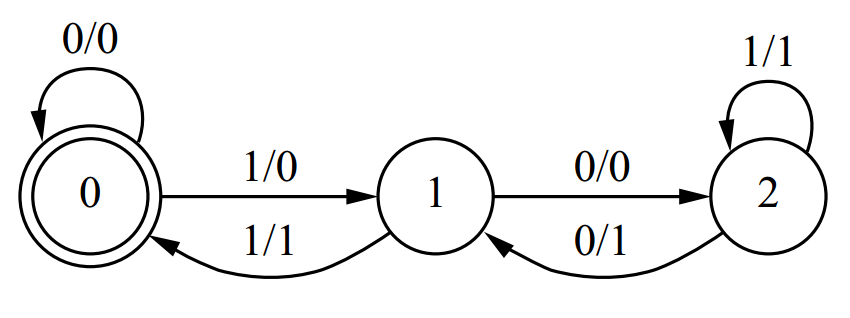
\includegraphics[scale=0.4]{images/fst.png}
  \caption{Zero or one NFA}
  \label{fig:fst}
\end{figure}


Regular expressions can be converted to automata \cite{aho1992foundations}, and FST is also an automata. To convert a regular expression over token to a FST we need two steps: The first is parsing the expression to a tree of matchers, the second is transfer the tree of matchers to the FST. We will introduce these two steps in next.

\subsection{Matchers in FST library}

In our library, a ``matcher'' could be a token to be matched, or a composition of other matchers. Our library supports syntax used in traditional regular expressions over strings. We list the syntax that the library supports in Table~\ref{tab:matchers}. The first column is the names of the matchers, the second column is the explanation of the function of the matchers, and third column is the their counterpart syntaxes of traditional regular expression. The RegexMatcher in our library is constructed with a regular expression, and the matcher matches any string that matches the regular expression in the matcher. We give examples of the syntax of these matchers in Table \ref{tab:matchers_example}.

\begin{table}[ht]
\caption{Matchers of our Library } % title of Table
\centering % used for centering table
\begin{tabular}{  | l | l | l |  }
 \hline
 Matcher Name        &  Function                                 & Counter Part of regex    \\
 \hline
 UnitMatcher       &  token is matches the it                  & character  in regex       \\
 \hline
 SequenceMatcher   &  A list of Matcher                        & sequence of characters       \\
  \hline
 QuestionMatcher   &  One or more of the preceding token       & ?       \\
  \hline
 StarMatcher       &  Zero or more of the preceding token      & *       \\
  \hline
 PlusMatcher       &  Zero or one of the preceding token       & +       \\
  \hline
 DotMatcher        &  Any token                                & .      \\
  \hline
 RegexMatcher      &  Any token matches the regular expression               &  N/A      \\
  \hline
\end{tabular}
\label{tab:matchers} % is used to refer this table in the text\section{Pipeline of Information Extraction}
\end{table}



\begin{table}[ht]
\caption{Matchers' Examples } % title of Table
\centering % used for centering table
\begin{tabular}{  | l |  l |  }
 \hline
 Matcher Name          & Example    \\
 \hline
 UnitMatcher         & DEGREE       \\
 \hline
 SequenceMatcher     & DE-LEVEL DEGREE       \\
  \hline
 QuestionMatcher     & DE-LEVEL (OR DE-LEVEL)?  DEGREE       \\
  \hline
 StarMatcher         & DE-LEVEL (, DE-LEVEL)*  DEGREE       \\
  \hline
 PlusMatcher         & DEGREE IN MAJOR +      \\
  \hline
 DotMatcher          & HAS . DEGREE      \\
  \hline
 RegexMatcher        & r``d-d'' years  \\
  \hline

\end{tabular}
\label{tab:matchers_example} % is used to refer this table in the text\section{Pipeline of Information Extraction}
\end{table}

The framework supports three styles of creating patterns: regular expression style, operator style and  object style. The second and third styles are flexible because developers can create their own matcher class to extend the feature of the library. We use examples to show how the three styles work. The most common style is defining pattern expression in a string, which is much like traditional regular expression.

\begin{framed}
\small
\noindent
The pattern is:  DE-LEVEL DEGREE ( IN  $\vert$  OF ) DT? MAJOR \\
The code is: \\
seqMatcher =parser.parse("DE-LEVEL DEGREE ( IN  $\vert$  OF ) DT? MAJOR")

\end{framed}

The second style is using algebraic operators to connect matchers, as follows:
\begin{framed}
\small
\noindent
The pattern is:  "DE-LEVEL DEGREE (IN $\vert$ OF) MAJOR" \\
The code is: \\
seqMatcher =  UnitMatcher("DE-LEVEL") +  UnitMatcher("DEGREE") + \\
\hspace{3cm} ( UnitMatcher("IN") $\vert$ UnitMatcher("OF" ) ) + UnitMatcher("MAJOR")

\end{framed}

We also could create a complex matcher in object-oriented programming style.

\begin{framed}
\small
\noindent
The pattern is:  "DE-LEVEL DEGREE (IN $\vert$ OF) MAJOR" \\
The code is: \\
matcher1 = UnitMatcher("DE-LEVEL") \\
matcher2 = UnitMatcher("DEGREE")  \\
matcher3 = UnitMatcher("IN")   \\
matcher4 = UnitMatcher("OF")   \\
matcher5 = UnitMatcher("MAJOR")  \\
matcher6 = AlternateMatcher([matcher3,matcher4])   \\
seqMatcher = SeqMatcher([matcher1, matcher2, matcher6, matcher5])

\end{framed}

The flexibility of the tool also comes from the fact that developers could determine which layer of the array should be matched, the original text, or labels in the first layer or labels in the second layer. Developers can assign lambda expression to the matcher's catching function, which defines how to get the matching input strings from the sentences, and out function, which defines what should be outputed. For example,  the labeled sentence is a sequence of arrays, each array includes the original text token and its labels in the other two layers, which is shown in table~\ref{tab:labeldsent}. To match the labeled sentence, we set the lambda expression for catching function to ``lambda x:x[2]'', and the out function to ``lambda x:x[1]'', which make the matcher match the label in second layer, and output the the value of semantic value in the first layer.


\subsection{Implementation of FST Library}
We use PLY(Python Lex-Yacc) as the grammar parser, which is a pure-Python implementation of the popular compiler construction tools lex and yacc. We defined  syntaxes of regular expression over tokens in the parser, which can parse the token regular expression to the tree structure of matchers.

We use the algorithm proposed by Thompson and Ken\cite{thompson1968programming} to construct the FST from the tree of matchers. Each matcher is a partial Nondeterministic Finite Automaton (NFA), which have one or more dangling arrows, pointing to nothing. We build the whole NFA by connecting the arrows of the partial NFAs. Different operator will have different structures of NFA, which is shown below:

The NFAs for matching single token is shown in Figure \ref{fig:nfa_single}.

\begin{figure}[htbp]
  \centering
  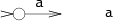
\includegraphics[scale=1]{images/single_token.png}
  \caption{Single Token NFA}
  \label{fig:nfa_single}
\end{figure}

The NFA for the concatenation $e_1e_2$ connects the final arrow of the $e_1$ machine to the start of the $e_2$ machine, as shown in Figure \ref{fig:nfa_cocat}.

\begin{figure}[htbp]
  \centering
  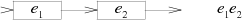
\includegraphics[scale=1]{images/concatenation_tokens.png}
  \caption{Concatenation NFA}
  \label{fig:nfa_cocat}
\end{figure}

The NFA for the alternation $e_1\mid e_2$ adds a new start state with a choice of either the $e_1$ machine or the $e_2$ machine, which is shown in Figure \ref{fig:nfa_alternation}.

\begin{figure}[htbp]
  \centering
  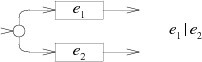
\includegraphics[scale=1]{images/alternation.png}
  \caption{Alternation NFA}
  \label{fig:nfa_alternation}
\end{figure}

The NFA for e? alternates the e machine with an empty path, which is shown in Figure \ref{fig:nfa_question}.

\begin{figure}[htbp]
  \centering
  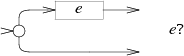
\includegraphics[scale=1]{images/question.png}
  \caption{Zero or one NFA}
  \label{fig:nfa_question}
\end{figure}

The NFA for e* uses the same alternation but loops a matching e machine back to the start, which is shown in Figure \ref{fig:nfa_star}.

\begin{figure}[htbp]
  \centering
  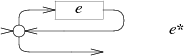
\includegraphics[scale=1]{images/star.png}
  \caption{Zero or more NFA}
  \label{fig:nfa_star}
\end{figure}

The NFA for e+ also creates a loop, but one that requires passing through e at least once, which is shown in Figure \ref{fig:nfa_plus}.
\begin{figure}[htbp]
  \centering
  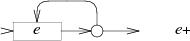
\includegraphics[scale=1]{images/plus.png}
  \caption{One or more NFA}
  \label{fig:nfa_plus}
\end{figure}

With above rules, we can convert the expression ``DL (, DL)*  (or DL)? DEGREE'' to an FST in Figure~\ref{fig:fst_pattern}.

\begin{figure}[htbp]
  \centering
  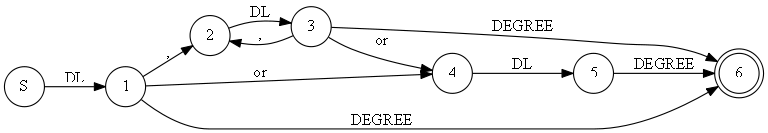
\includegraphics[scale=0.6]{images/test_tokenre2_6.png}
  \caption{Finite Automata Transducers}
  \label{fig:fst_pattern}
\end{figure}

In this chapter we have introduced how we extracted the information from the resumes and job descriptions, and the implementation details of the pattern matching library, regular expression over tokens. We can get the models of resumes and job descriptions through the procedure described in this chapter. In next chapter, we will discuss how our system searches and ranks job models by resume models.
